%TCIDATA{Version=5.00.0.2570}
%TCIDATA{LaTeXparent=0,0,Presentation-CAFE-displacement-subdoc.tex}
% $Id: Presentation-subdoc-replicability.tex 1765 2015-11-11 12:50:51Z lv39 $
% $URL: https://forge.cornell.edu/svn/repos/lv39_papers/BigThinkPresentations/UQAM2015/Presentation/Presentation-subdoc-replicability.tex $
\section{Replicability}



\begin{frame}
	\frametitle{Replication of research results}
	\begin{block}{Critical element of science}
		\begin{itemize}
			\item Replication of methods, data inputs, computational environment is a critical element of the scientific approach
			\item Journals, funding agencies (in the U.S.) have been moving to making archiving of inputs to scientific results more robust, even mandatory
		\end{itemize}
	\end{block}
\end{frame}


\begin{frame}
	\frametitle{The problem}
	\begin{block}{Good intentions, costly access}
		\begin{quote}
			``researchers could submit programs that [...] research assistants
			would run. Alternatively, researchers wishing to work directly with the data could come and
			work on the Institute's premises. ''
		\end{quote}
	\end{block}
	\pause
	\begin{block}{Uncertain access}
		\begin{quote}
			``Data [...] is proprietary and owned by the Alachua
			County, Florida School District. The corresponding author [...] holds the deidentified
			dataset [...] and will provide copies to
			authors who receive written permission from the Alachua County Public Schools.''
		\end{quote}
	\end{block}
	\pause
	\begin{block}{No access}
		\begin{quote}
			Some do not provide any information on access.	
		\end{quote}
	\end{block}
\end{frame}




\begin{frame}
	\frametitle{Not a new problem}
	\begin{columns}
		\begin{column}{.7\textwidth}
			\begin{block}{Econometrica}
				``In its first issue, the editor of Econometrica (1933), Ragnar Frisch, noted
				the importance of publishing data such that readers could fully explore
				empirical results.  Publication of data, however, was discontinued early in
				the journal's history.  [...]  The journal arrived full-circle in late 2004 when Econometrica
				adopted one of the more stringent policies on availability of data and
				programs.
			\end{block}
			\tiny \href{http://www.econometricsociety.org/submissions.asp\#4}{http://www.econometricsociety.org/submissions.asp\#4} as cited in \href{http://research.stlouisfed.org/wp/2005/2005-014.pdf}{Anderson et al (2005)}
		\end{column}
		\begin{column}{.3\textwidth}
			\href{http://www.jstor.org/stable/i332704}{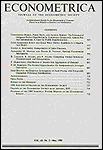
\includegraphics[width=\textwidth]{econometrica-vol1.png}}
		\end{column}
	\end{columns}
\end{frame}

\begin{frame}
	\frametitle{Problem will become worse}
	\begin{block}{Increased use of restricted-access data}
		\begin{itemize}
			\item Archiving (curation) of input data is complicated
			\item Knowledge discovery is complicated
		\end{itemize}
	\end{block}
\end{frame}
\begin{frame}
	\frametitle{Decline in the use of classic public-use data}
	\centering
	%\includepdf[pages={1-2}]{Chetty-1-2-Slides.pdf}
	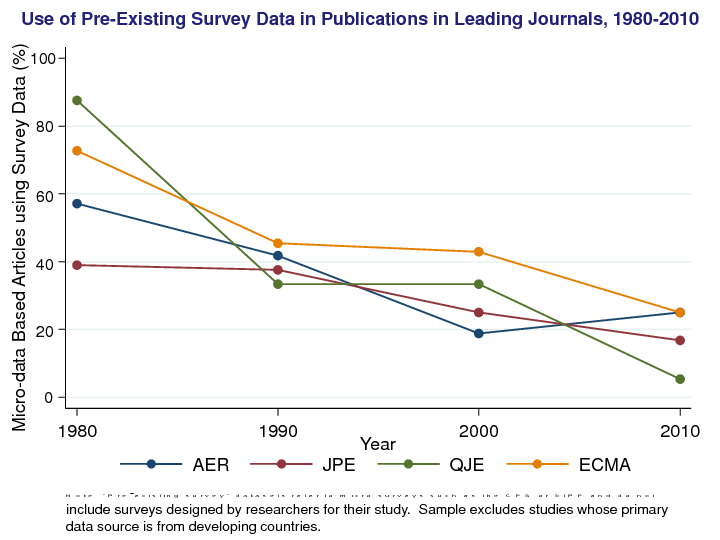
\includegraphics[width=0.7\paperwidth]{ChettySlide1}
\end{frame}

\begin{frame}
	\frametitle{Increase in the use of administrative data in economics}
	\centering
	%\includepdf[pages={1-2}]{Chetty-1-2-Slides.pdf}
	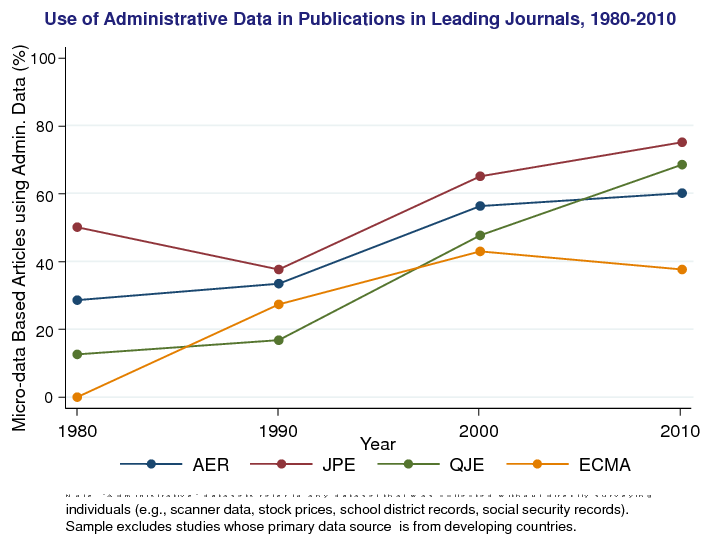
\includegraphics[width=0.7\paperwidth]{ChettySlide2}
\end{frame}


\begin{frame}
	\frametitle{Results from the LDI Replication Lab}
	\begin{block}{Undergraduate research team}
		\begin{itemize}
			\item Census of articles in the American Economic Journal: Applied Economics (2010, 2011, 2013)
			\item Each article is analyzed for availability of replication archive (as required by journal!) 
			\item If data and programs are available, reproducibility is tested. 
		\end{itemize}
	\end{block}
\end{frame}

% extract from Replication.Rnw

\begin{frame}
	\frametitle{Some very preliminary results}
	
	\centering
	\begin{table}[!htbp] \centering 
		\caption{Replication Success} 
		\label{} 
		\begin{tabular}{@{\extracolsep{5pt}} ccccc} 
			\\[-1.8ex]\hline 
			\hline \\[-1.8ex] 
			& Yes & No & Partial & Sum \\ 
			\hline \\[-1.8ex] 
			2010 & $10$ & $19$ & $6$ & $35$ \\ 
			2011 & $12$ & $20$ & $4$ & $36$ \\ 
			2013 & $15$ & $12$ & $11$ & $38$ \\ 
			\hline \\[-1.8ex] 
			
			\bf		Total &\bf $37$ &\bf $51$ &\bf $21$ &\bf $109$ \\ 
			\hline \\[-1.8ex] 
		\end{tabular} 
	\end{table} 
\end{frame}

\begin{frame}
	\frametitle{Some very preliminary results}
	% Table created by stargazer v.5.2 by Marek Hlavac, Harvard University. E-mail: hlavac at fas.harvard.edu
	% Date and time: Mon, Nov 09, 2015 - 09:22:20 PM
	\centering \small
	\begin{table}[!htbp] 
		\caption{Reason for Replication Failure} 
		\label{} 
		\begin{tabular}{@{\extracolsep{5pt}} cccccc} 
			\\[-1.8ex]\hline 
			\hline \\[-1.8ex] 
			& Missing  & Corrupted  & Code  & Missing &  \\ 
			& Data     & Data       & Error & Code    & Sum \\ 
			\hline \\[-1.8ex] 
			2010 & $15$ & $1$ & $1$ & $2$ & $19$ \\ 
			2011 & $15$ & $1$ & $1$ & $3$ & $20$ \\ 
			2013 & $12$ & $0$ & $0$ & $0$ & $12$ \\ 
			\hline \\[-1.8ex] 
			\bf Total &\bf $42$ &\bf $2$ &\bf $2$ &\bf $5$ &\bf $51$ \\ 
			\hline \\[-1.8ex] 
		\end{tabular} 
	\end{table} 
\end{frame}


\begin{frame}
	\frametitle{Some very preliminary results}
	\centering
	% Table created by stargazer v.5.2 by Marek Hlavac, Harvard University. E-mail: hlavac at fas.harvard.edu
	% Date and time: Tue, Nov 10, 2015 - 01:24:18
	\begin{table}[!htbp] \centering 
		\caption{Reason for Missing Data} 
		\label{} 
		\begin{tabular}{ ccccccc} 
			\\[-1.8ex]\hline 
			\hline \\[-1.8ex] 
			&\multicolumn{3}{c}{Administrative}&\multicolumn{2}{c}{Private} &  \\ 
			\cline{2-4}\cline{5-6}
			&  local &  National &  Regional &  Commercial &  Other & Sum \\ 
			\hline \\[-1.8ex] 
			2010 & $2$ & $8$ & $0$ & $4$ & $3$ & $17$ \\ 
			2011 & $2$ & $8$ & $4$ & $1$ & $0$ & $15$ \\ 
			2013 & $2$ & $2$ & $1$ & $4$ & $2$ & $11$ \\ 
			\hline \\[-1.8ex] 
			Total & $6$ & $18$ & $5$ & $9$ & $5$ & $43$ \\ 
			\hline \\[-1.8ex] 
		\end{tabular} 
	\end{table} 
\end{frame}


\begin{frame}
	\frametitle{Some very preliminary results}
	% Table created by stargazer v.5.2 by Marek Hlavac, Harvard University. E-mail: hlavac at fas.harvard.edu
	% Date and time: Tue, Nov 10, 2015 - 01:24:18
	\begin{table}[!htbp] \centering 
		\caption{Type of Access to Confidential Data} 
		\label{} 
		\begin{tabular}{ cccccc} 
			\\[-1.8ex]\hline 
			\hline \\[-1.8ex] 
			&  &\multicolumn{2}{c}{Informal} & No  &  \\ 
			& Formal & w/ Commitment & w/o Commitment &  Info & Sum \\ 
			\hline \\[-1.8ex] 
			2010 & $2$ & $3$ & $9$ & $3$ & $17$ \\ 
			2011 & $2$ & $0$ & $10$ & $3$ & $15$ \\ 
			2013 & $1$ & $2$ & $8$ & $0$ & $11$ \\ 
			\hline \\[-1.8ex] 
			\bf	Total & $5$ & $5$ & $27$ & $6$ & $43$ \\ 
			\hline \\[-1.8ex] 
		\end{tabular} 
	\end{table} 
\end{frame}



\begin{frame}
	\frametitle{Not limited to one journal}
	\begin{block}{NIH-funded research}
		\begin{itemize}
			\item article is open-access
			\item not clear about data access
		\end{itemize}
	\end{block}
\end{frame}

\tikzset{
	arr/.style={->,blue,very thick},
	lbl/.style={draw,blue,very thick},
	shadowed/.style={preaction={transform canvas={shift={(2pt,-1pt)}},draw=gray,very thick}},
}
\begin{frame}
	\frametitle{A small anonymous example}
	\begin{tikzpicture}
	\node[draw=none,drop shadow={shadow scale=0.97,
		top color=black,bottom color=gray,
		shadow xshift=3pt,
		shadow yshift=-2pt,
		opacity=0.9}]
	at (1,1) {\fcolorbox{black}{white}{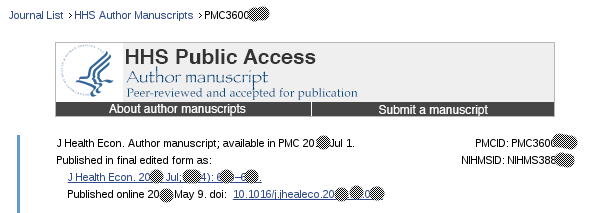
\includegraphics[scale=0.5]{Selection_031}}}; \pause
	%
	\node[draw=none,drop shadow={shadow scale=0.95,
		top color=black,bottom color=gray,
		shadow xshift=3pt,
		shadow yshift=-2pt,
		opacity=0.9}]
	at (1,1) {\fcolorbox{black}{white}{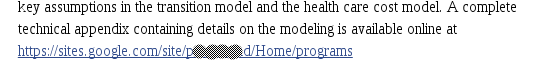
\includegraphics[scale=0.5]{Selection_030}}};
	\pause
	\node[draw=none,drop shadow={shadow scale=0.93,
		top color=black,bottom color=gray,
		shadow xshift=3pt,
		shadow yshift=-2pt,
		opacity=0.9}]
	at (1,1) {\fcolorbox{black}{white}{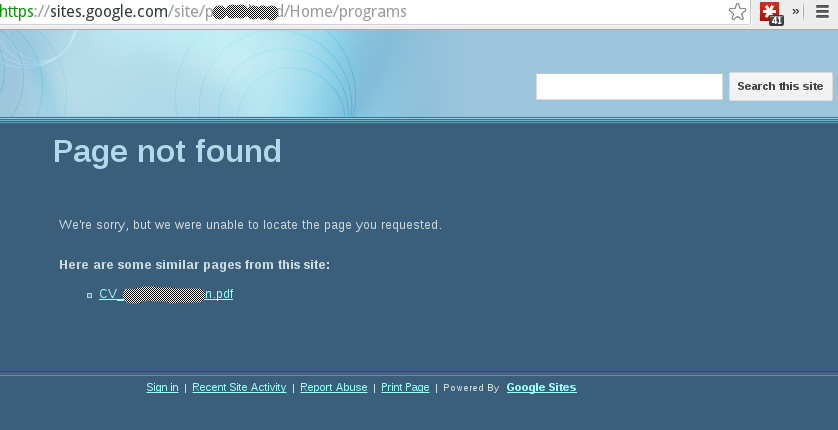
\includegraphics[scale=0.25]{Selection_032}}};
	\pause
	\node[draw=none,drop shadow={shadow scale=0.93,
		top color=black,bottom color=gray,
		shadow xshift=3pt,
		shadow yshift=-2pt,
		opacity=0.9}]
	at (1,1) {\fcolorbox{black}{white}{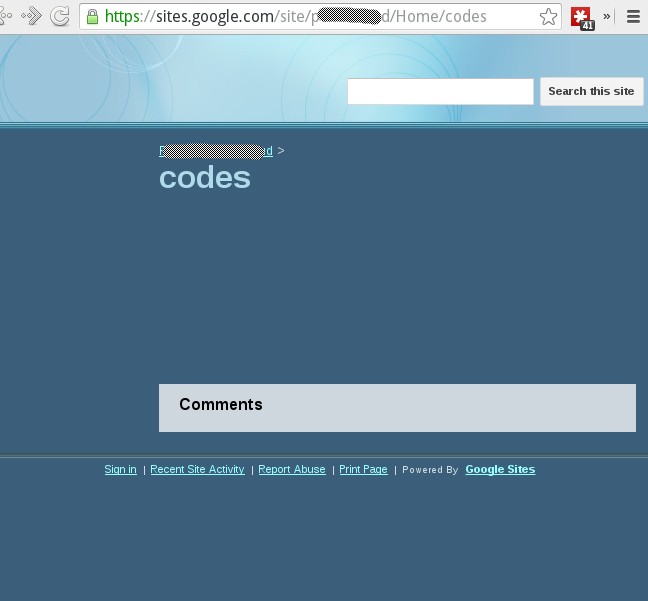
\includegraphics[scale=0.25]{Selection_029}}};
	\end{tikzpicture}
	
\end{frame}

\begin{frame}
	\frametitle{Not limited to economics}
	\begin{block}{Nature, 2012}
		``Many of the emerging `big data' applications come from private sources that are inaccessible to other researchers. The data source may be hidden, compounding problems of verification, as well as concerns about the generality of the results.''\\
	\end{block}
	{\tiny (Huberman, Nature 482, 308 (16 February 2012) \href{http://dx.doi.org/10.1038/482308d}{doi:10.1038/482308d})}
	\begin{block}{Other domains}
		\begin{itemize}
			\item Biology (genetics data, chemical compounds)
			\item Computer science (search records, single-firm examples)
		\end{itemize}
	\end{block}
\end{frame}


\begin{frame}
	\frametitle{Non-federal confidential data}
	States, school districts, private companies, academic and private surveys: need a place to live to be re-used.
	\begin{block}{Options}
		\begin{itemize}
			\item openICPSR \url{https://www.openicpsr.org/}
			\item Harvard Dataverse \url{https://dataverse.harvard.edu/} {\footnotesize (1,315\ DV, 59,530 DS)}
			\item Ontario Council of University Libraries: \url{http://dataverse.scholarsportal.info/dvn/} {\footnotesize (64\ DV, 5,289 files)}
		\end{itemize}
	\end{block}
	Hinges on compatibility of data deposit rules, laws, regulations, etc.
\end{frame}


%\begin{frame}
%	\frametitle{Can we influence this process?}
%	\begin{block}{Data repositories have the technology to receive deposits}
%		\begin{itemize}
%			\item Underutilized
%			\item When integrated into journal workflows, useless (blobs of unstructured ZIP files)
%		\end{itemize}
%	\end{block}
%	\begin{block}{Journals can require data citations}
%		\begin{itemize}
%			\item Review process scrutinizes \textit{article} citations
%			\item Would be easy to enforce \textit{data} citations
%		\end{itemize}
%	\end{block}
%\end{frame}

\begin{frame}
	\frametitle{Data citations}
	\begin{block}{Examples} {\tiny  \footnotesize \tt
		\begin{quote}
			Deschenes, Elizabeth Piper, Susan Turner, and Joan Petersilia. \textbf{Intensive Community Supervision in Minnesota, 1990-1992: A Dual Experiment in Prison Diversion and Enhanced Supervised Release} [Computer file]. ICPSR06849-v1. Ann Arbor, MI: Inter-university Consortium for Political and Social Research [distributor], 2000. \alert<2>{doi:10.3886/ICPSR06849}
		\end{quote}
		\begin{quote}
			Abowd, John M.; Vilhuber, Lars, 2014, "\textbf{Replication data for: National estimates of gross employment and job flows from the Quarterly Workforce Indicators with demographic and industry detail}", \alert<2>{doi:10.7910/DVN/27923}, Harvard Dataverse [Distributor], V2
		\end{quote}[\href{http://www.icpsr.umich.edu/icpsrweb/ICPSR/curation/citations.jsp}{src}]}
	\end{block}
\end{frame}

\begin{frame}
	\frametitle{So we know how to deposit and cite data...}
	\pause
\begin{beamercolorbox}[sep=8pt,center]{title}
	\usebeamerfont{title}... except nobody does it...
\end{beamercolorbox}

\end{frame}

\begin{frame}
	\frametitle{We didn't do it...}
	\begin{block}{Abowd and Vilhuber (2011)}
   \begin{tikzpicture}
   \node[draw=none,drop shadow={shadow scale=0.97,
   	top color=black,bottom color=gray,
   	shadow xshift=3pt,
   	shadow yshift=-2pt,
   	opacity=0.9}]
   at (1,1) {\fcolorbox{black}{white}{
\includegraphics[scale=0.5]{Selection_126}}}; \pause
   %
   \node[draw=none,drop shadow={shadow scale=0.95,
   	top color=black,bottom color=gray,
   	shadow xshift=3pt,
   	shadow yshift=-2pt,
   	opacity=0.9}]
   at (1,1) {\fcolorbox{black}{white}{
\includegraphics[scale=0.5]{Selection_125}}};
   \pause
   \node[draw=none,drop shadow={shadow scale=0.93,
   	top color=black,bottom color=gray,
   	shadow xshift=3pt,
   	shadow yshift=-2pt,
   	opacity=0.9}]
   at (1,1) {\fcolorbox{black}{white}{
\includegraphics[scale=0.5]{Selection_124}}};
   \end{tikzpicture}		
	\end{block}
\end{frame}

\begin{frame}
	\frametitle{Then we archived it better...}
	\begin{block}{... at Harvard Dataverse}
   \begin{tikzpicture}
   \node[draw=none,drop shadow={shadow scale=0.97,
   	top color=black,bottom color=gray,
   	shadow xshift=3pt,
   	shadow yshift=-2pt,
   	opacity=0.9}]
   at (1,1) {\fcolorbox{black}{white}{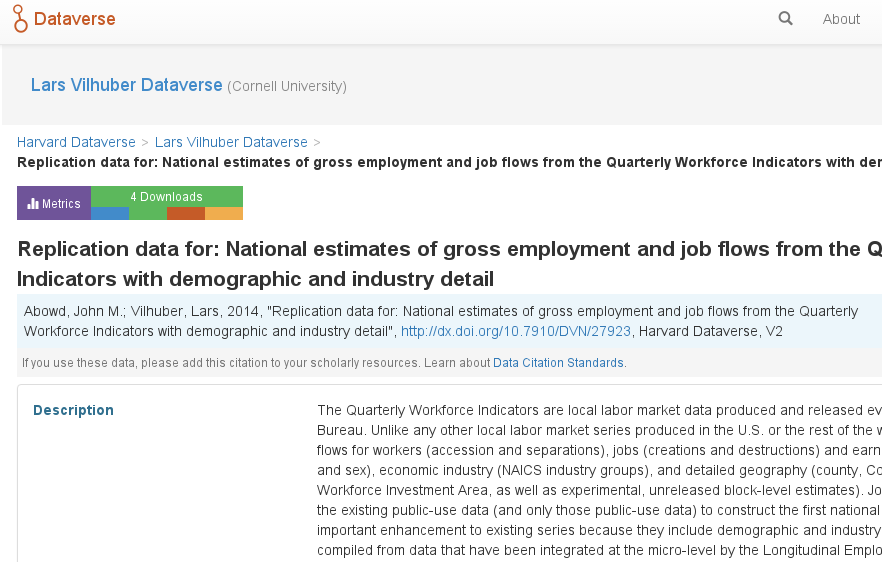
\includegraphics[scale=0.3]{Selection_128}}}; \pause
   %
   \node[draw=none,drop shadow={shadow scale=0.95,
   	top color=black,bottom color=gray,
   	shadow xshift=3pt,
   	shadow yshift=-2pt,
   	opacity=0.9}]
   at (1,1) {\fcolorbox{black}{white}{
\includegraphics[scale=0.3]{Selection_129}}};\pause
   %
   \node[draw=none,drop shadow={shadow scale=0.95,
   	top color=black,bottom color=gray,
   	shadow xshift=3pt,
   	shadow yshift=-2pt,
   	opacity=0.9}]
   at (1,1) {\fcolorbox{black}{white}{
\includegraphics[scale=0.3]{Selection_129_hilight}}};
   \end{tikzpicture}		
	\end{block}
\end{frame}

\begin{frame}{Provenance}
	\begin{block}{The provenance problem}
		``data provenance, one kind of metadata, pertains to the derivation history of a
		data product starting from its original sources'' [...]  ``from it, one can ascertain
		the quality of the data base and its ancestral data and derivations, track back sources
		of errors, allow automated reenactment of derivations to update the data, and provide 
		attribution of data sources'' 
	\end{block}
	{\tiny Simmhan, Plale, and Gannon, ``A survey of data provenance in e-science,'' ACM Sigmod Record, 2005}
\end{frame}


\begin{frame}{Provenance (cont)}
	\begin{block}{PROV model}
		W3C PROV Model  based in the notions of 
		\begin{enumerate}
			\item \textbf{entities} that are physical, digital, and conceptual
			things in the world; 
			\item \textbf{activities} that are dynamic aspects of the world that change and
			create entities; and 
			\item \textbf{agents} that are responsible for activities. 
			\item  a set of \textbf{relationships} that can exist be-
			tween them that express attribution,. delegation, derivation, etc.
		\end{enumerate}
	\end{block}
	\begin{block}{PROV and Metadata}
		Not (currently) a ``native'' component of DDI
	\end{block}
\end{frame}

%\begin{frame}{Incorporating PROV (LBD)}
%	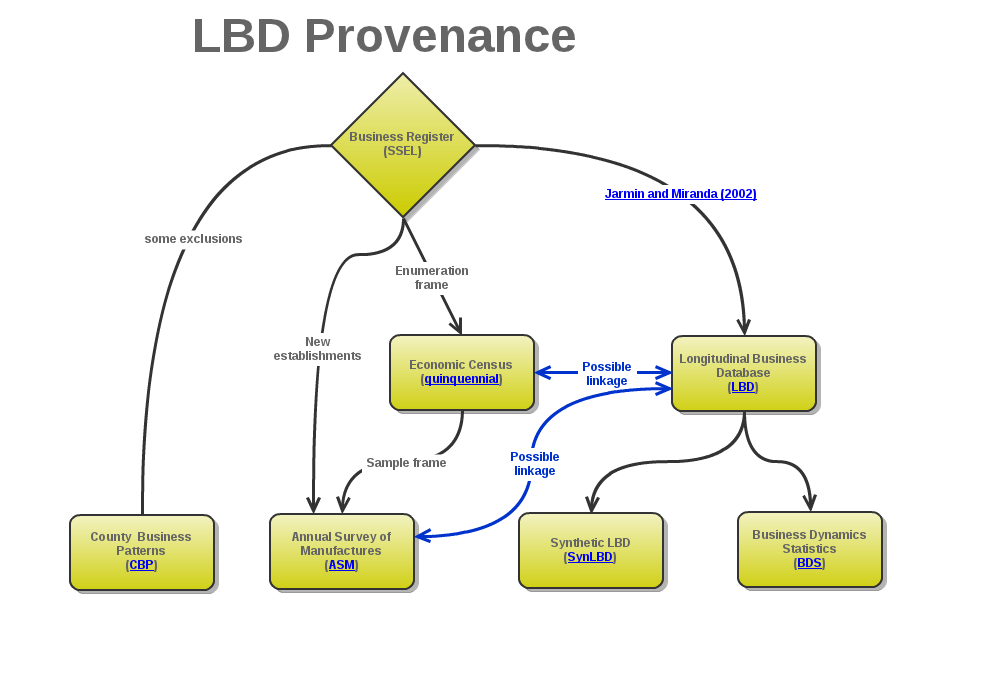
\includegraphics[width=\textwidth]{LBD_Provenance.png}
%\end{frame}
%
%\begin{frame}{Incorporating PROV (LBD)}
%	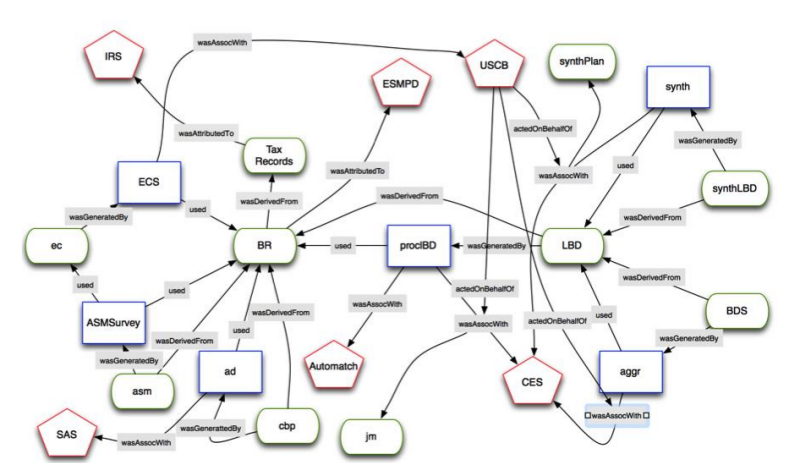
\includegraphics[width=0.9\textwidth]{LBD_Prov_simplified.png}
%\end{frame}


\begin{frame}
	\frametitle{Provenance for research}
	\begin{block}{Sample research activity with full provenance}

	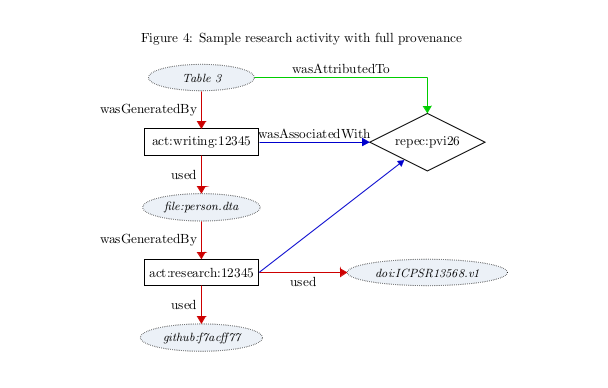
\includegraphics[scale=0.5]{tikz-authorship-example}
	\end{block}
\end{frame}


\begin{frame}
	\frametitle{Provenance for research}
	\begin{block}{Sample research activity with simple provenance}
		\centering
		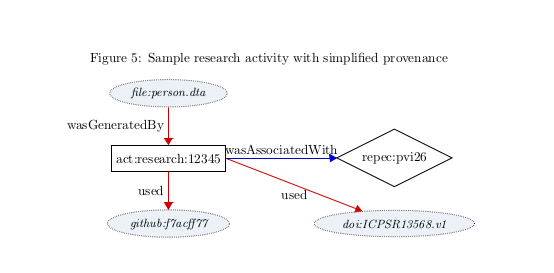
\includegraphics[scale=0.5]{tikz-authorship-example-simple}
	\end{block}
\end{frame}

%\begin{frame}
%\begin{beamercolorbox}[sep=8pt,center]{title}
%	\usebeamerfont{title}Putting it together
%\end{beamercolorbox}
%\end{frame}
%
%
%\begin{frame}
%	\begin{beamercolorbox}[sep=8pt,center]{title}
%		\usebeamerfont{title}Easy editing of all elements of data description
%	\end{beamercolorbox}
%\end{frame}
%
%\begin{frame}
%	\centering		
%	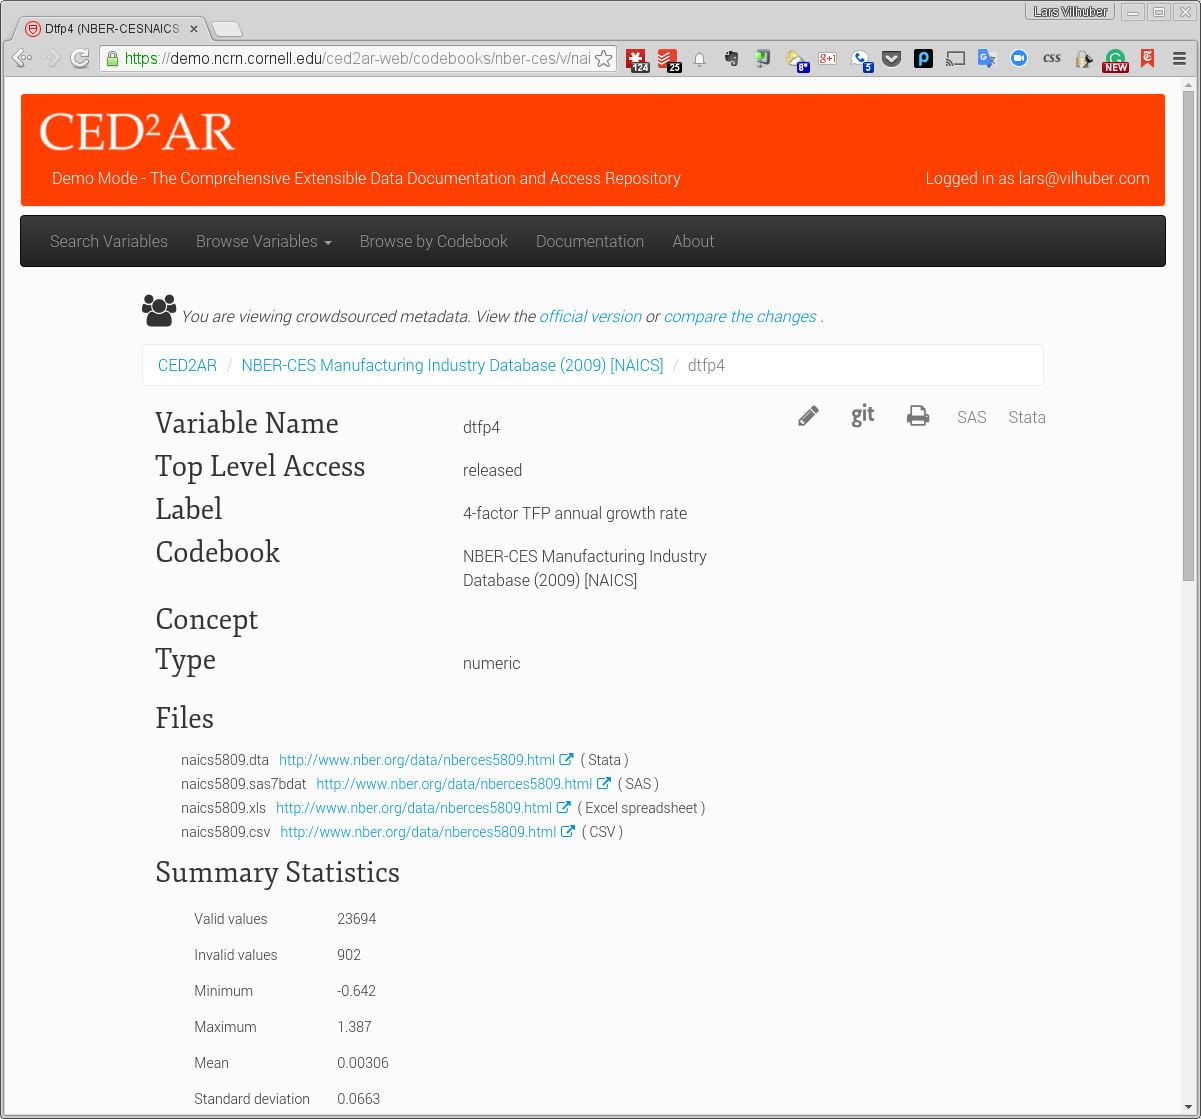
\includegraphics[height=\textheight]{Selection_133}
%\end{frame}
%
%\begin{frame}
%	\centering		
%	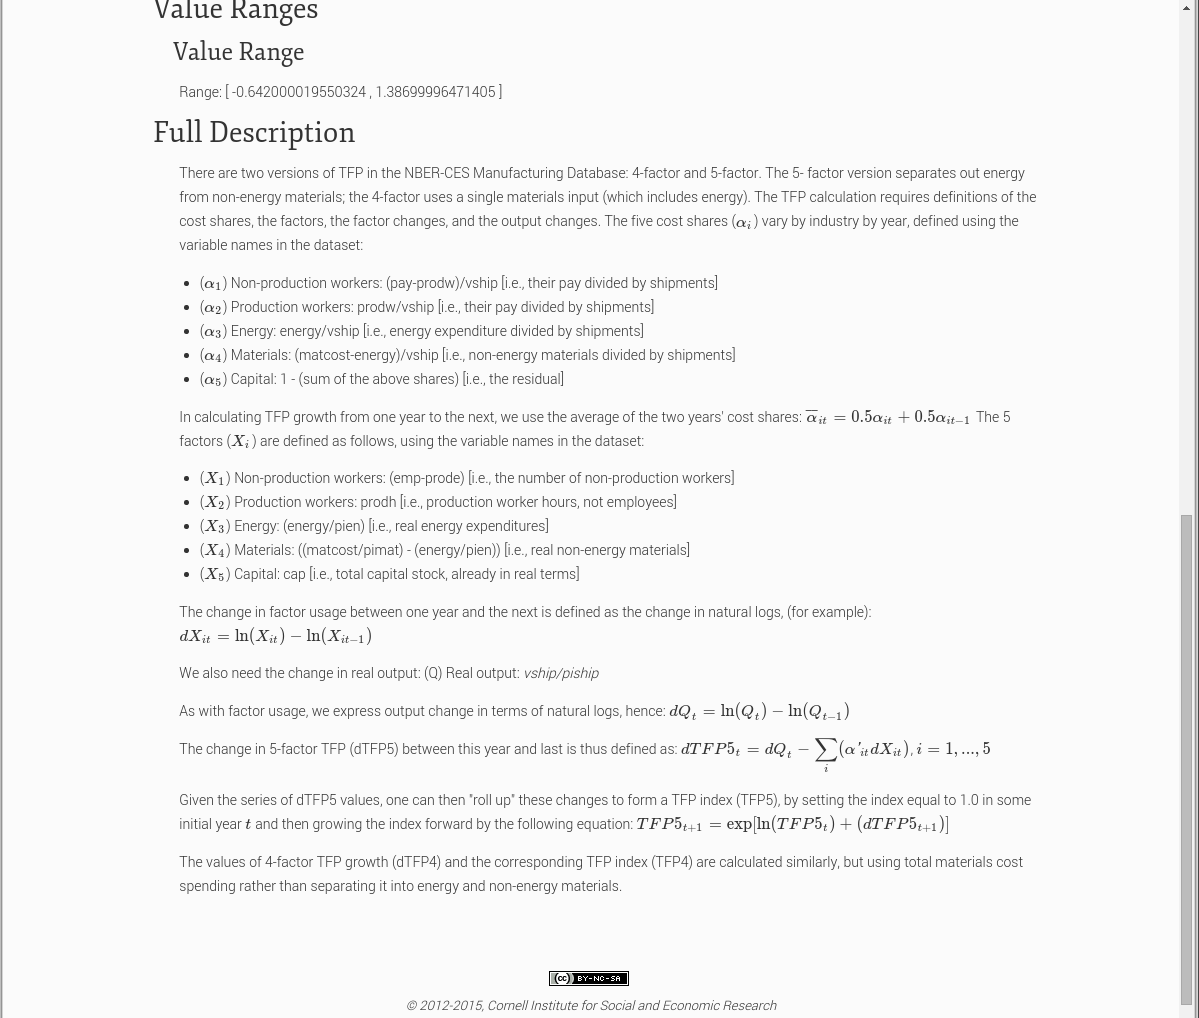
\includegraphics[height=\textheight]{Selection_134}
%\end{frame}
%
%\begin{frame}
%	\centering		
%	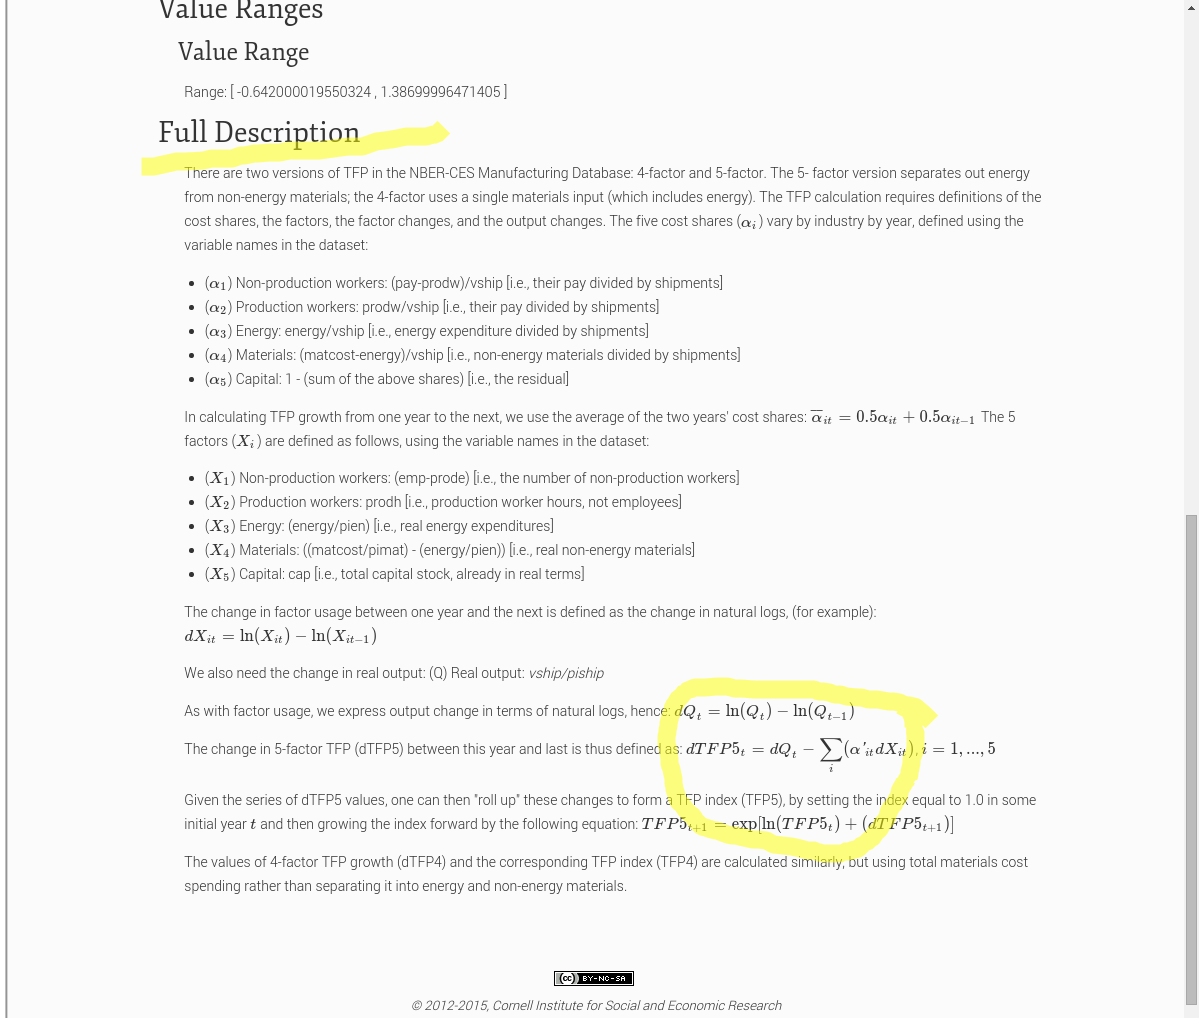
\includegraphics[height=\textheight]{Selection_134_hilite}
%\end{frame}
%
%\begin{frame}
%	\frametitle{Lacking from other implementations}
%	\begin{block}{... such as}
%		\centering
%		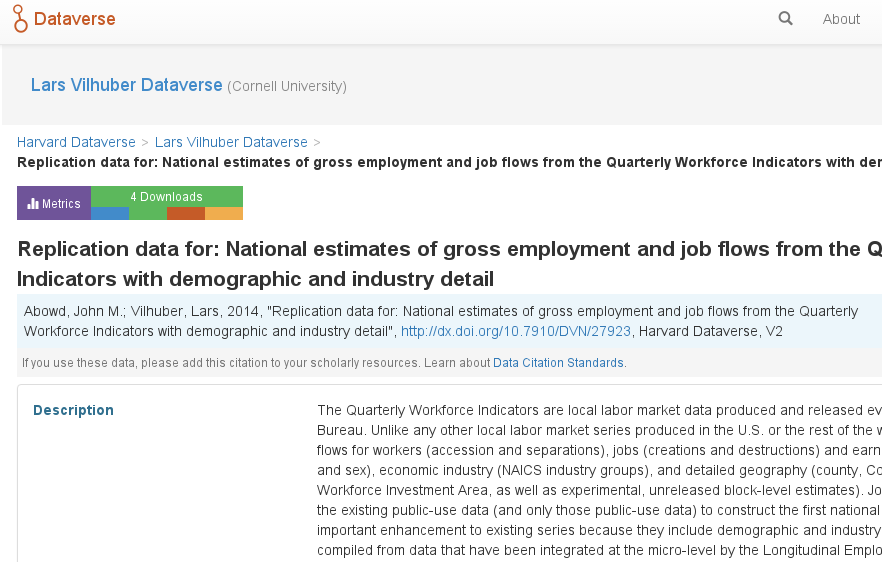
\includegraphics[scale=0.5]{Selection_128}
%		
%	\end{block}
%\end{frame}
%
%\begin{frame}
%	\begin{beamercolorbox}[sep=8pt,center]{title}
%		\usebeamerfont{title}Editing of provenance
%	\end{beamercolorbox}
%\end{frame}
%
%
%\begin{frame}
%\centering		
%		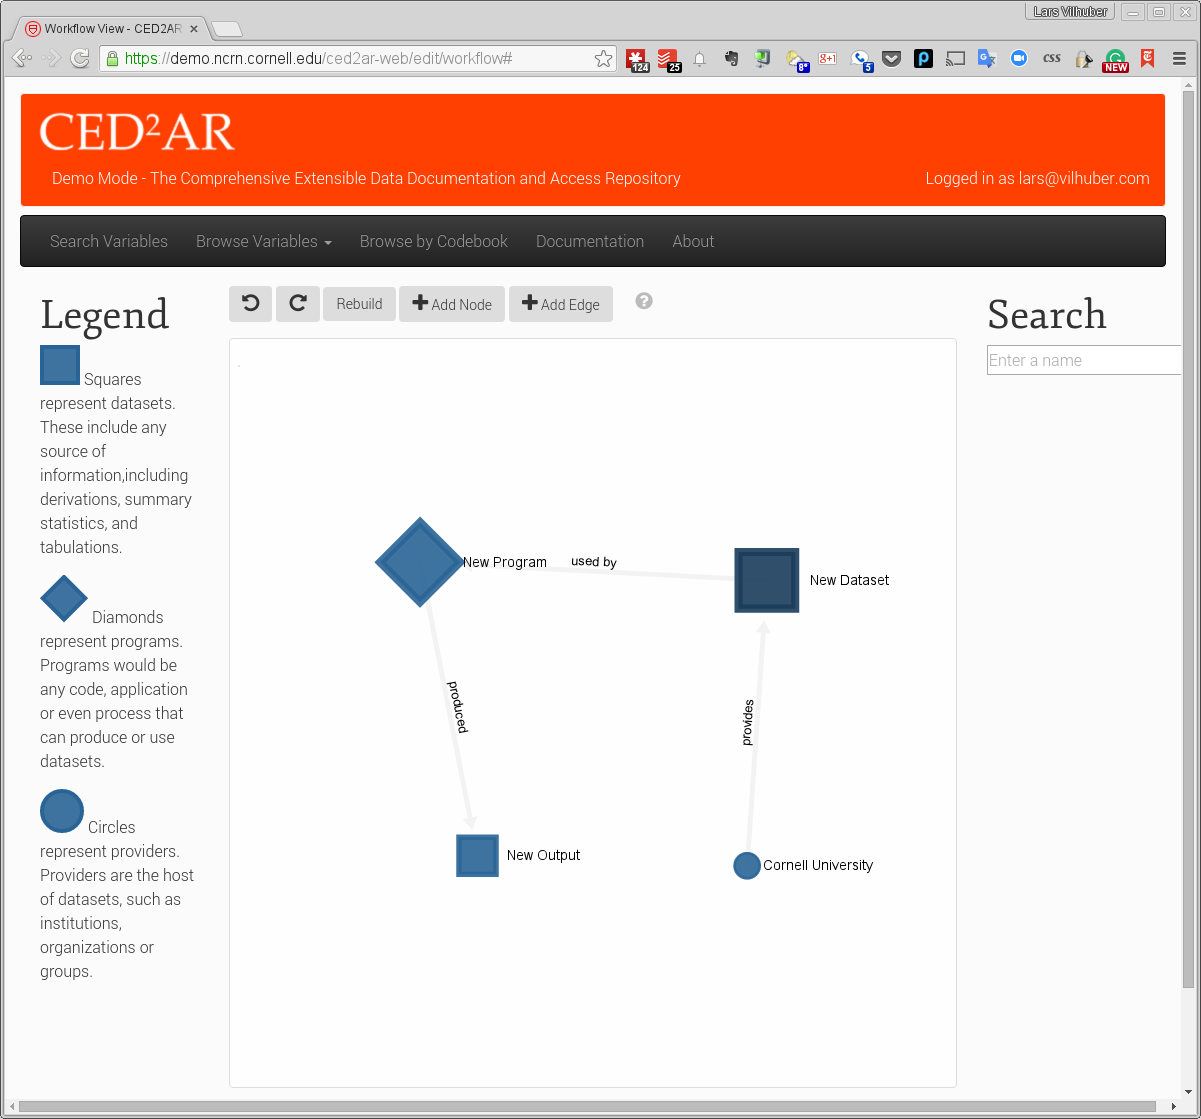
\includegraphics[height=\textheight]{Selection_132}
%\end{frame}
%
%\begin{frame}
%	\frametitle{Possibilities}
%	\begin{block}{Enhance journal or working paper archives}
%		\begin{itemize}
%			\item Capture the essential elements of programs, data, and how they are linked
%		\end{itemize}
%	\end{block}
%	\begin{block}{Machine readable!}
%	Because the metadata is structured, actionable data ensues
%	\begin{itemize}
%		\item Reproducible archives!
%		\item Disclosure avoidance requests (Census RDC, German RDC require such documentation, but currently unstructured)
%	\end{itemize}
%	\end{block}
%\end{frame}
%
%\begin{frame}
%	\frametitle{Additional elements}
%	\begin{block}{Ex-post linking of articles and data}
%		\centering
%
\includegraphics[scale=0.3]{Selection_129_hilight}
%	\end{block}
%\end{frame}
%
%\begin{frame}
%	\frametitle{Additional elements}
%	\begin{block}{Ex-post linking of articles and data}
%	\begin{itemize}
%		\item Lacking from existing repositories of both data and bibliographies
%		\item Exposure of data providers
%		\item Sometimes manually (labor intensive) performed by data archives (e.g. ICPSR)
%		\item Not currently done on RePEc
%	\end{itemize}
%	\end{block}
%\end{frame}
%
%
%\begin{frame}
%	\frametitle{Crowd-sourcing data provenance}
%	\begin{block}{Let other people contribute}
%   \begin{tikzpicture}
%   \node[draw=none,drop shadow={shadow scale=0.97,
%   	top color=black,bottom color=gray,
%   	shadow xshift=3pt,
%   	shadow yshift=-2pt,
%   	opacity=0.9}]
%   at (1,1) {\fcolorbox{black}{white}{
\includegraphics[scale=0.3]{Selection_135}}}; \pause
%   %
%   \node[draw=none,drop shadow={shadow scale=0.95,
%   	top color=black,bottom color=gray,
%   	shadow xshift=3pt,
%   	shadow yshift=-2pt,
%   	opacity=0.9}]
%   at (1,1) {\fcolorbox{black}{white}{
\includegraphics[scale=0.3]{Selection_136}}};
%   \end{tikzpicture}		
%	\end{block}
%\end{frame}
%
%\begin{frame}
%	\frametitle{Crowd-sourcing data provenance}
%	\begin{block}{Work in progress: on RePEc}
%	\begin{itemize}
%		\item Deploy a graphical interface that maps co-author networks, genealogy...
%		\item ... and data provenance 
%		\begin{itemize}
%			\item incoming: what data did an article use? (LDI Replication workshop scaled up)
%			\item outgoing: what data did an article create? (Better tracking of replication archives, or the National QWI example)
%		\end{itemize}
%		\item Users (or contributors!) can ``claim'' data, or if hosted on a data repository.
%	\end{itemize}
%	\end{block}
%\end{frame}
%
%\begin{frame}
%	\frametitle{Other methods and efforts}
%	\begin{block}{Similar linkage efforts}
%		\begin{itemize}
%			\item \href{http://www.rd-switchboard.org/}{RD-Switchboard}, based on \href{https://orcid.org/}{ORCID} IDs
%			\item Direct DataCite/ORCID efforts
%		\end{itemize}
%	\end{block}
%\end{frame}
%
%\begin{frame}
%\begin{beamercolorbox}[sep=8pt,center]{title}
%	\usebeamerfont{title}... we've only barely started...
%\end{beamercolorbox}
%\end{frame}

%%% Local Variables:
%%% mode: latex
%%% End:
